\documentclass[landscape]{article}

\pagenumbering{gobble}
\usepackage{tikz}
\usetikzlibrary{calc,shapes,positioning,fit}

\usetikzlibrary{arrows}
\newcommand{\midarrow}{\tikz \draw[-triangle 90] (0,0) -- +(.1,0);}
\usepackage{bm}
\newcommand{\Rr}{\mathcal{R}}
\newcommand{\Tt}{\mathcal{T}}

\usepackage{amsmath,graphicx}
\newcommand{\ubar}[1]{\mkern2mu\underline{\mkern-2mu #1\mkern-2mu}\mkern2mu}
\newcommand{\ubm}[1]{\ubar{\bm{#1}}}
% \newcommand{\ubmr}[2]{\ubar{\bm{#1}}^{#2}}

\begin{document}
\begin{figure}[!t]
  \centering
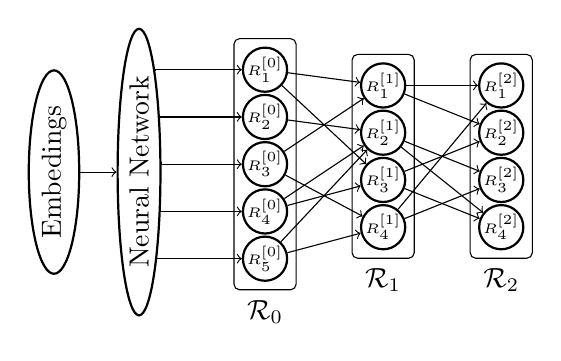
\begin{tikzpicture}
    \tikzstyle{enode} = [thick, draw=black, ellipse, inner sep = 2pt,  align=center]
    \tikzstyle{cnode} = [thick, draw=black, circle, inner sep = 0.0pt,  align=center]
    \tikzstyle{nnode} = [thick, rectangle, rounded corners = 0pt,draw,inner sep = 2pt]
    \begin{scope}[xshift=-4cm, yshift=0cm, scale=1.0]

    \begin{scope}[xshift=-1cm, yshift=-1.3cm, scale=0.6]
      \node[enode, rotate=90] (em) at (-1.8,0) {Embedings};
      \node[enode, rotate=90] (nn) {Neural Network};
    \end{scope}
    % level0 regions
    \begin{scope}[scale=0.6]
    \node[cnode] (r01) at (1, 0) {\tiny$R_1^{[0]}$};
    \node[cnode] (r02) at (1, -1) {\tiny$R_2^{[0]}$};
    \node[cnode] (r03) at (1, -2) {\tiny$R_3^{[0]}$};
    \node[cnode] (r04) at (1, -3) {\tiny$R_4^{[0]}$};
    \node[cnode] (r05) at (1, -4) {\tiny$R_5^{[0]}$};
    \node[label=below:$\Rr_0$, draw,rounded corners = 2pt, inner sep=1mm, fit=(r01) (r05)] {};
  \end{scope}

  \draw[->] (nn.351.9) |- (r01);
  \draw[->] (nn.340) |- (r02);
  \draw[->] (nn.295) |- (r03);
  \draw[->] (nn.210) |- (r04);
  \draw[->] (nn.191) |- (r05);
  \draw[->] (em) -- (nn);

    % level 1 regions
    \begin{scope}[xshift=1.5cm, yshift=-0.2cm, scale=0.6]
    \node[cnode] (r11) at (1, 0) {\tiny$R_1^{[1]}$};
    \node[cnode] (r12) at (1, -1) {\tiny$R_2^{[1]}$};
    \node[cnode] (r13) at (1, -2) {\tiny$R_3^{[1]}$};
    \node[cnode] (r14) at (1, -3) {\tiny$R_4^{[1]}$};
    \node[label=below:$\Rr_1$, draw, rounded corners = 2pt, inner sep=1mm, fit=(r11) (r14)] {};
    \end{scope}


    % level 1 regions
    \begin{scope}[xshift=3cm, yshift=-0.2cm, scale=0.6]
    \node[cnode] (r21) at (1, 0) {\tiny$R_1^{[2]}$};
    \node[cnode] (r22) at (1, -1) {\tiny$R_2^{[2]}$};
    \node[cnode] (r23) at (1, -2) {\tiny$R_3^{[2]}$};
    \node[cnode] (r24) at (1, -3) {\tiny$R_4^{[2]}$};
    \node[label=below:$\Rr_2$, draw, rounded corners = 2pt, inner sep=1mm, fit=(r21) (r24)] {};
    \end{scope}

    \draw[->] (r01) -- (r11);
    \draw[->] (r03) -- (r11);

    \draw[->] (r02) -- (r12);
    \draw[->] (r04) -- (r12);
    \draw[->] (r05) -- (r12);

    \draw[->] (r01) -- (r13);
    \draw[->] (r04) -- (r13);

    \draw[->] (r03) -- (r14);
    \draw[->] (r05) -- (r14);


    \draw[->] (r11) -- (r21);
    \draw[->] (r14) -- (r21);

    \draw[->] (r11) -- (r22);
    \draw[->] (r13) -- (r22);

    \draw[->] (r12) -- (r23);
    \draw[->] (r14) -- (r23);

    \draw[->] (r12) -- (r24);
    \draw[->] (r13) -- (r24);


    \end{scope}
  \end{tikzpicture}


\end{figure}


\end{document}
%%% Local Variables:
%%% mode: latex
%%% TeX-master: t
%%% End:
